\documentclass{article}
\title{Algorithm Homework}
\author{Tai Jiang}
\date{October 2023}
\usepackage{amsmath}
\usepackage{tikz}
\usepackage{color}
\begin{document}
  \maketitle
  \tableofcontents
  \pagenumbering{gobble}
  \newpage
  \pagenumbering{arabic}
  \section{Show that the solution of  $ T \left(n\right) = T \left(\left\lceil n/2 \right\rceil\right) + 1  $ is $ O \left( \lg n \right)  $ .}
    \paragraph{Origin}:
      \subparagraph{Exercise}4.3-2
      \subparagraph{Page}87
    \paragraph{Answer}:

  That can build a recursion tree to visualize how this recurrence works:

  \begin{enumerate}
    \item Start with $ T \left(n\right) $ at the top.
    \item At each level of the tree, we have $ T \left( \left\lceil n/2 \right\rceil \right) + 1 $.
    \item The tree branches into two subproblems, one with size $ \left\lceil n/2 \right\rceil $ and another with size $ \left\lceil n/2 \right\rceil $.
  \end{enumerate}

  The tree might look like Figure \ref{fig:tree1}.

  \begin{figure}[h!]
    \centering
    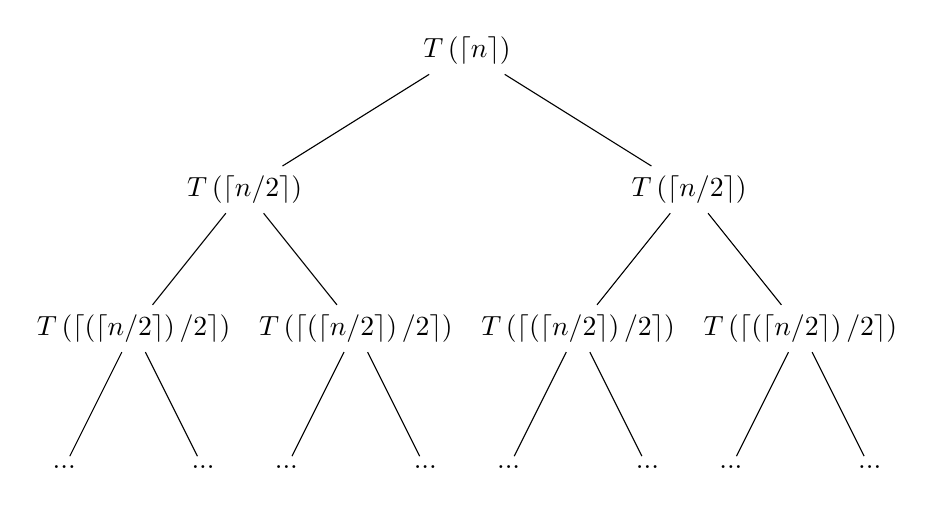
\begin{tikzpicture}
      [level distance=50px,
       level 1/.style={sibling distance=160px},
       level 2/.style={sibling distance=80px},
       level 3/.style={sibling distance=50px}]
      \node {$ T \left(\left\lceil n \right\rceil\right) $}
        child {node {$ T \left(\left\lceil n/2 \right\rceil\right) $}
          child {node {$ T \left(\left\lceil  \left(\left\lceil n/2 \right\rceil\right) /2 \right\rceil\right) $}
            child {node {...}}
            child {node {...}}
          }
          child {node {$ T \left(\left\lceil  \left(\left\lceil n/2 \right\rceil\right) /2 \right\rceil\right) $}
            child {node {...}}
            child {node {...}}
          }
        }
        child {node {$ T \left(\left\lceil n/2 \right\rceil\right) $}
          child {node {$ T \left(\left\lceil  \left(\left\lceil n/2 \right\rceil\right) /2 \right\rceil\right) $}
            child {node {...}}
            child {node {...}}
          }
          child {node {$ T \left(\left\lceil  \left(\left\lceil n/2 \right\rceil\right) /2 \right\rceil\right) $}
            child {node {...}}
            child {node {...}}
          }
        };
    \end{tikzpicture}
    \caption{Recursion Tree.}
    \label{fig:tree1}
  \end{figure}

  At each level, the size of the problem is divided by 2, and we keep going until the size becomes 1 (or less, in which case we stop). The depth of the tree will be the number of times we can halve n until it becomes 1. So it's the number of times we can take $ \left\lceil n/2 \right\rceil $ until $ \left\lceil n/2 \right\rceil \leq  1 $.
  
  At each step, we're taking the ceiling of half of the previous value, which is effectively dividing it by 2. We continue this process until the value is less than or equal to 1. So, let k be the number of steps it takes for $ \left\lceil n/2 \right\rceil $ to become 1, look like equation \eqref{eq:tree1}.

  \begin{equation}
    \frac{\left\lceil n/2 \right\rceil}{2^k}  \leq 1
    \label{eq:tree1}
  \end{equation}

  Then sovle for k, look like equation \eqref{eq:tree2}:
  
  \begin{equation}
    \begin{aligned}
      \frac{n}{2^k} \leq 1 \\
      n \leq 2^k \\
      \lg n \leq k
    \end{aligned}
    \label{eq:tree2}
  \end{equation}

  The depth of the recursion tree is $ O(\lg n) $, which means the algorithm has a time complexity of $ O(\lg n) $. So the solution of  $ T \left(n\right) = T \left(\left\lceil n/2 \right\rceil\right) + 1 $ is indeed $ O(\lg n) $.

  \section{Use a recursion tree to determine a good asymptotic upper bound on the recurrence $ T \left(n\right) = 4T \left( n/2 + 2 \right) + n  $. Use the substitution method to verify your answer.}
    \paragraph{Origin}:
      \subparagraph{Exercise}4.4-3
      \subparagraph{Page}93
    \paragraph{Answer}:

    That can build a recursion tree to visualize how this recurrence works:

    \begin{enumerate}
      \item Start with $ T \left(n\right)  $ at the top.
      \item At each level of the tree, we have 4 subproblems of size $ T \left( n/2 + 2 \right) + n  $.
      \item The cost of each level is n.
    \end{enumerate}

    The tree might look like Figure \ref{fig:tree2}.

  \begin{figure}[h!]
    \centering
    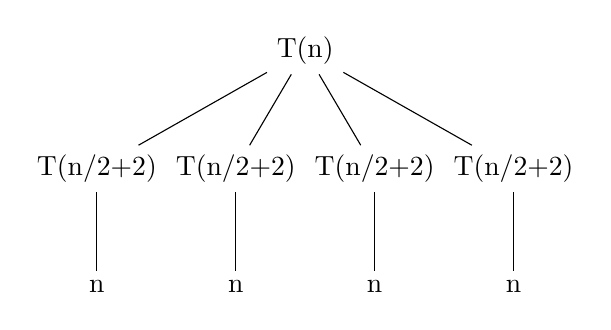
\begin{tikzpicture}[sibling distance=50px]
      \node {T(n)}
        child {node {T(n/2+2)}
          child {node {n}}
        }
        child {node {T(n/2+2)}
          child {node {n}}
        }
        child {node {T(n/2+2)}
          child {node {n}}
        }
        child {node {T(n/2+2)}
          child {node {n}}
        };

    \end{tikzpicture}
    \caption{Recursion Tree.}
    \label{fig:tree2}
  \end{figure}

  At each level, we have 4 subproblems of size T(n/2 + 2), and each subproblem incurs a cost of n. The number of levels in the tree will depend on how quickly the subproblem size decreases.

  The subproblem size is equation \eqref{eq:q2_1}:

  \begin{equation}
    T(n) = 4T(n/2 + 2) + n
    \label{eq:q2_1}
  \end{equation}

  The subproblem size is n/2 + 2, so we calculate the subproblem size for the next level by equation \eqref{eq:q2_2}:
  \begin{equation}
    \begin{aligned}
      T(n/2 + 2) &= 4T((n/2 + 2)/2 + 2) + n/2 + 2 \\
      &= 4T(n/4 + 1 + 2) + n/2 + 2 \\
      &= 4T(n/4 + 3) + n/2 + 2      
    \end{aligned}
    \label{eq:q2_2}
  \end{equation}

  At each level, we are adding 2 to the subproblem size. Therefore, at level k, the subproblem size will be $ n/(2^k) + 2k $.

  Now, we want to find the level where the subproblem size becomes a constant, $ n/(2^k) + 2k = C for some constant C $, calculate the k look like equation \eqref{eq:q2_3}.

  \begin{equation}
    \begin{aligned}
      n/(2^k) + 2k &= C \\
      n/(2^k) &= C - 2k \\
      2^k &= n/(C - 2k) \\
      k &= \lg (n/(C - 2k))
    \end{aligned}
    \label{eq:q2_3}
  \end{equation}

  C is a constant. The number of levels in the recursion tree is $ O(\lg n) $.

  The cost at each level in the recursion tree is equation \eqref{eq:q2_4}:

  \begin{equation}
    \begin{aligned}
      \text{At level 0:}& \quad n \\
      \text{At level 1:}& \quad 4 * n/2 = 2n \\
      \text{At level 2:}& \quad 4 * (n/4) = n \\
      ... \\
      \text{At level k:}& \quad (4^k) * (n/(2^k)) = (n/2^k) * (4^k) = C * 4^k
    \end{aligned}
    \label{eq:q2_4}
  \end{equation}

  Summing up the costs of all levels(Equation \eqref{eq:q2_5}):

  \begin{equation}
    T(n) = n + 2n + 4n + ... + C * 4^k
    \label{eq:q2_5}
  \end{equation}

  This is a geometric series, and its sum can be bounded by(Equation \eqref{eq:q2_6}):

  \begin{equation}
    T(n) \leq  n * (1 - 4^(k+1))/(1 - 4)
    \label{eq:q2_6}
  \end{equation}

  Since $k = O(\lg(n))$, $4^(k+1)$ is polynomial in n. Therefore, T(n) is O(n).

  verify this result using the substitution method:

  Assume that $T(m) \leq  km - p$ for some positive constants k and p, where m < n(Equation \eqref{eq:q2_7}).

  \begin{equation}
    \begin{aligned}
      T(n) = 4T(n/2 + 2) + n \\
        \leq  4(k(n/2 + 2) - p) + n \\
        = 2kn - 4k + 4n - 4p + n \\
        = (2k + 5)n - 4k - 4p
    \end{aligned}
    \label{eq:q2_7}
  \end{equation}

  Find k and p such that $(2k + 5)n - 4k - 4p \leq  kn - p$.
  
  This holds if $2k + 5 \leq k and -4k - 4p \leq -p$.
  
  Solving these inequalities(Equation \eqref{eq:q2_8}):

  \begin{equation}
    \begin{aligned}
      2k + 5 &\leq k \\
      k &\leq -5 \\
      -4k - 4p &\leq -p \\
      -4k &\leq 0\\
      k &\geq  0
    \end{aligned}
    \label{eq:q2_8}
  \end{equation}

  Since we can't find k and p that satisfy these inequalities, our initial assumption that $ T(m) \leq km - p$ for m < n is incorrect.

  Therefore, T(n) is not $O(n^k)$ for any positive constant k. Instead, as shown earlier, T(n) is O(n).
  
  \section{Can the master method be applied to the recurrence $ T(n) = 4T(n/2) + n^2 \lg n $? Why or why not? Give an asymptotic upper bound for this recurrence.}

  \paragraph{Origin}:
    \subparagraph{Exercise}4.5-4
    \subparagraph{Page}97
  \paragraph{Answer}:

  The master theorem can be applied to recurrence

  To apply the master theorem, we need to check whether f(n) satisfies the following conditions for some constant $\epsilon  > 0$:

  \begin{enumerate}
    \item If $ f(n) = O(n^{log_{b} a - \epsilon } ) $, for some $\epsilon > 0$, then $T(n) = \Theta (n^{log_{b}a})$.
    \item If $ f(n) = \Theta(n^{log_{b}a}) $, then $ T(n) = \Theta(n^{log_{b} a}  \lg n) $.
    \item If $ f(n) = \Omega (n^{log_{b}a + \epsilon}) $, for some $\epsilon > 0$, and if $a f(n/b) \leq k * f(n)$ for some k < 1 and sufficiently large n, then $T(n) = \Theta(f(n))$.
  \end{enumerate}

  The asymptotic upper bound for the given recurrence relation $T(n) = 4T(n/2) + n^2 * \lg n = O(n^2)$.

  \section{Use indicator random variables to compute the expected value of the sum of n dice.}

  \paragraph{Origin}:
    \subparagraph{Exercise}5.2-3
    \subparagraph{Page}122
  \paragraph{Answer}:

Let $X_i$ be the random variable that is 1 if the i-th die shows a particular face (1, 2, 3, 4, 5, or 6), and 0 otherwise.

The sum of n dice can then be expressed as the sum of these indicator variables:

$ S = X_1 + X_2 + X_3 + ... + X_n $

Now, we can calculate the expected value of S:

$ E(S) = E(X_1) + E(X_2) + E(X_3) + ... + E(X_n) $

Since each die is fair, the probability of each face (1, 2, 3, 4, 5, or 6) appearing on a single die is 1/6, and the expected value of each indicator variable is:

$ E(X_i) = 1 * P(X_i = 1) + 0 * P(X_i = 0) = 1 * (1/6) + 0 * (5/6) = 1/6 $

Now, you can sum up the expected values of the individual indicators:

$ E(S) = E(X_1) + E(X_2) + E(X_3) + ... + E(X_n) = (1/6) + (1/6) + (1/6) + ... + (1/6) = (n/6) $

So, the expected value of the sum of n dice is (n/6).



  \section{Use indicator random variables to solve the following problem, which is known as the hat-check problem. Each of n customers gives a hat to a hat-check person at a restaurant. The hat-check person gives the hats back to the customers in a random order. What is the expected number of customers who get back their own hat?}

  \paragraph{Origin}:
    \subparagraph{Exercise}5.2-4
    \subparagraph{Page}122
  \paragraph{Answer}:

  Let $X_i$ be an indicator random variable for the i-th customer, where:

  $X_i = 1$ if the i-th customer gets their own hat back.
  $X_i = 0$ if the i-th customer does not get their own hat back.
  
  The probability that the i-th customer gets their own hat back is 1/n, as there are n hats and they are returned in a random order. Therefore, we have:
  
  $E(X_i) = P(X_i = 1) = 1/n$
  
  Now, let's define a random variable Y as the total number of customers who get their own hat back. Y is the sum of the indicator random variables for each customer:
  
  $Y = X_1 + X_2 + X_3 + ... + X_n$
  
  Now, we can find the expected value of Y using linearity of expectation:
  
  $E(Y) = E(X_1 + X_2 + X_3 + ... + X_n)$
  
  Using the linearity of expectation, we can write this as:
  
  $E(Y) = E(X_1) + E(X_2) + E(X_3) + ... + E(X_n)$
  
  Since each customer's indicator random variable has the same expected value (1/n), we can simplify further:
  
  $E(Y) = (1/n) + (1/n) + (1/n) + ... + (1/n) (n times)$
  
  $E(Y) = (1/n) * n = 1$
  
  So, the expected number of customers who get back their own hat is 1. This result may be surprising, but it's a classic result of the hat-check problem. On average, one customer is expected to get their own hat back, while the others get hats belonging to other customers.


\end{document}